%% Begin slides template file
\documentclass[11pt,t,usepdftitle=false,aspectratio=169]{beamer}
%% ------------------------------------------------------------------
%% - aspectratio=43: Set paper aspect ratio to 4:3.
%% - aspectratio=169: Set paper aspect ratio to 16:9.
%% ------------------------------------------------------------------

\usetheme[nototalframenumber,foot,logo]{uibk}

\title[Segfault Slayer]{Progress Update 3: Segfault Slayer}

\author[Schmölz Lukas, Schöpf Emanuel, Schweigl Dominik]{\textbf{Schmölz Lukas}, Schöpf Emanuel, Schweigl Dominik}

\headerimage{3}

\begin{document}

\section{Bookmark Title}
\subsection{Overview}


\begin{frame}
	\frametitle{Minimaps }

	\textbf{Initial Scribbles:}

	\begin{columns}[T]
		\begin{column}{0.5\textwidth}
			\begin{center}
				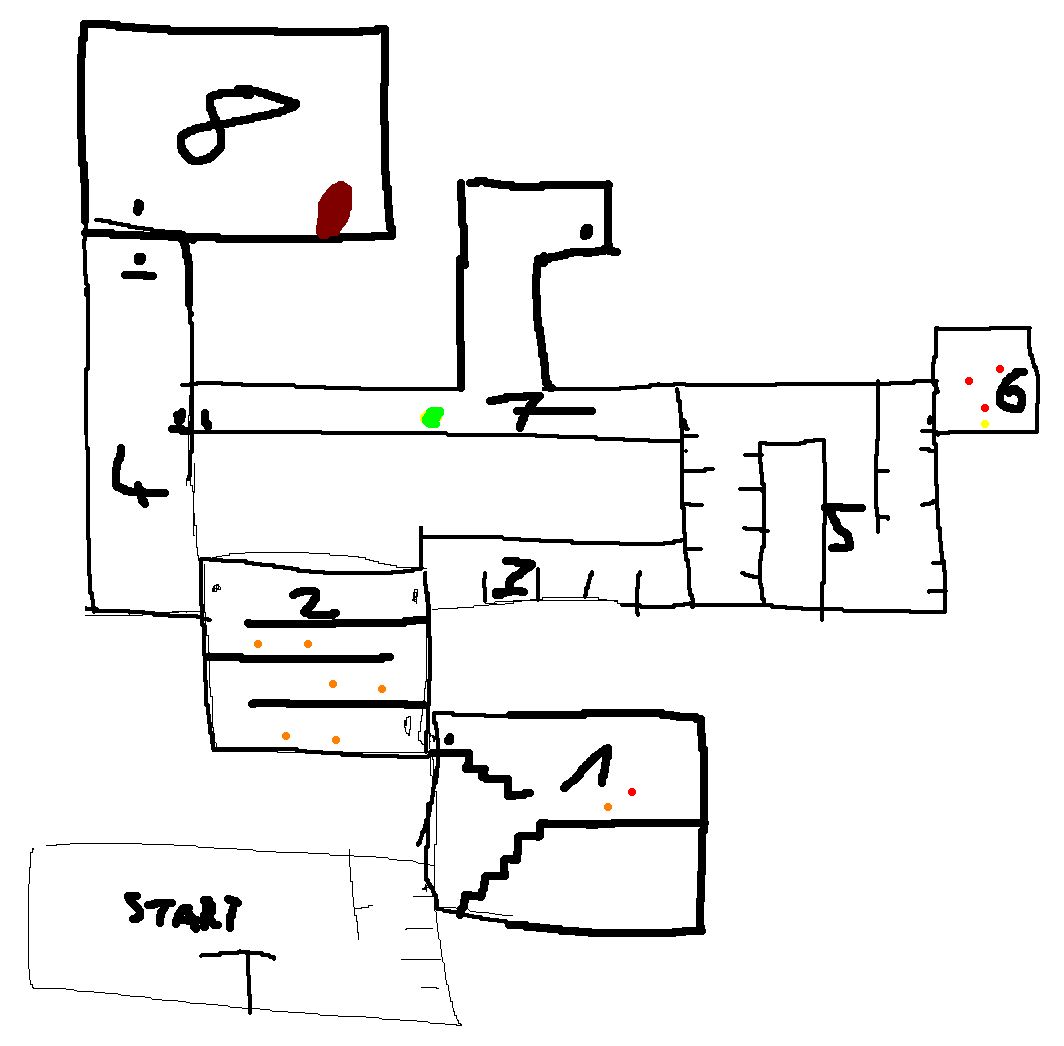
\includegraphics{_images/first_area_scribble.png}
			\end{center}
		\end{column}
		\begin{column}{0.5\textwidth}
			\begin{center}
				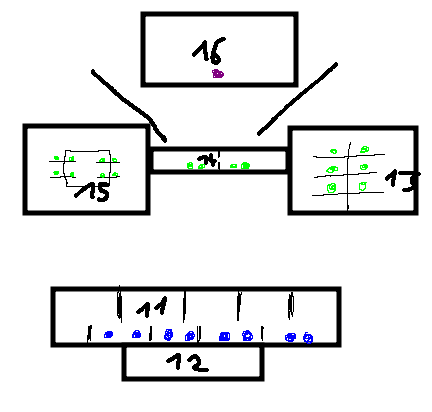
\includegraphics{_images/second_area_scribble.png}
			\end{center}
		\end{column}
	\end{columns}
\end{frame}

\begin{frame}
	\frametitle{Minimaps }

	\textbf{current: }

	\text{(work in progress)}
	\vspace{-1em}
	\begin{columns}[T]
		\begin{column}{0.5\textwidth}
			\begin{center}
				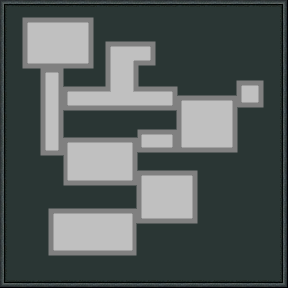
\includegraphics{_images/minimap1.png}
			\end{center}
		\end{column}
		\begin{column}{0.5\textwidth}
			\begin{center}
				
\includegraphics{_images/minimap2.png}
			\end{center}
		\end{column}
	\end{columns}
\end{frame}

\begin{frame}
	\frametitle{Data Design}

	\textbf{Flexibility \& Extensibility}

	\text{some examples:}
	\begin{itemize}
		\item Loot Drops
		\item Door Locked
		\item Room Minimap FloatRect
	\end{itemize}

	\begin{columns}[T]
		\begin{column}{0.5\textwidth}
			\begin{center}

				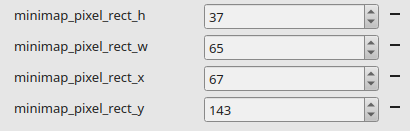
\includegraphics{_images/Tiled_props_room.png}
			\end{center}
		\end{column}
		\begin{column}{0.5\textwidth}
			\begin{center}

				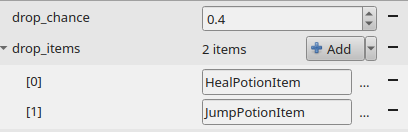
\includegraphics{_images/Tiled_props_enemy.png}
			\end{center}
		\end{column}
	\end{columns}
\end{frame}

\begin{frame}
	\frametitle{Saving and Loading World}

	\begin{columns}[T]
		\begin{column}{0.5\textwidth}
			\begin{center}
				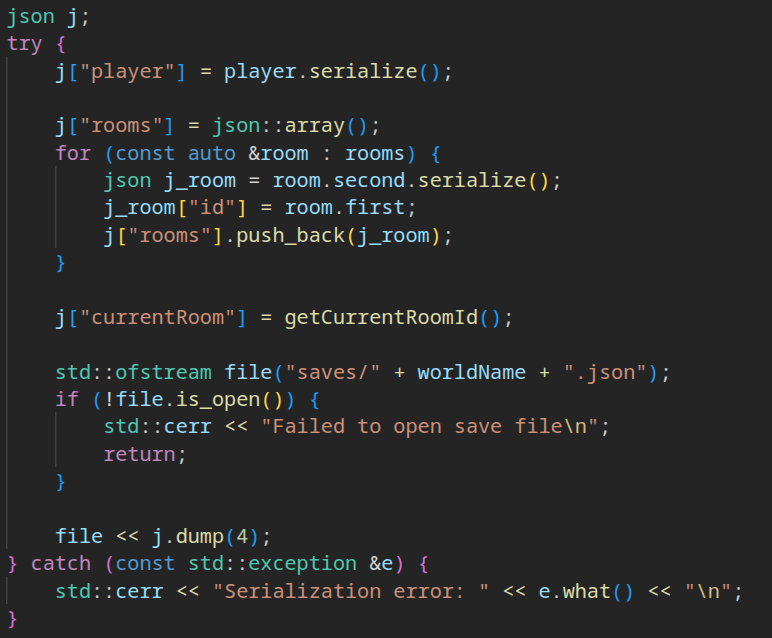
\includegraphics{_images/saveWorldData.png}
			\end{center}
		\end{column}
		\begin{column}{0.5\textwidth}
			\begin{center}
				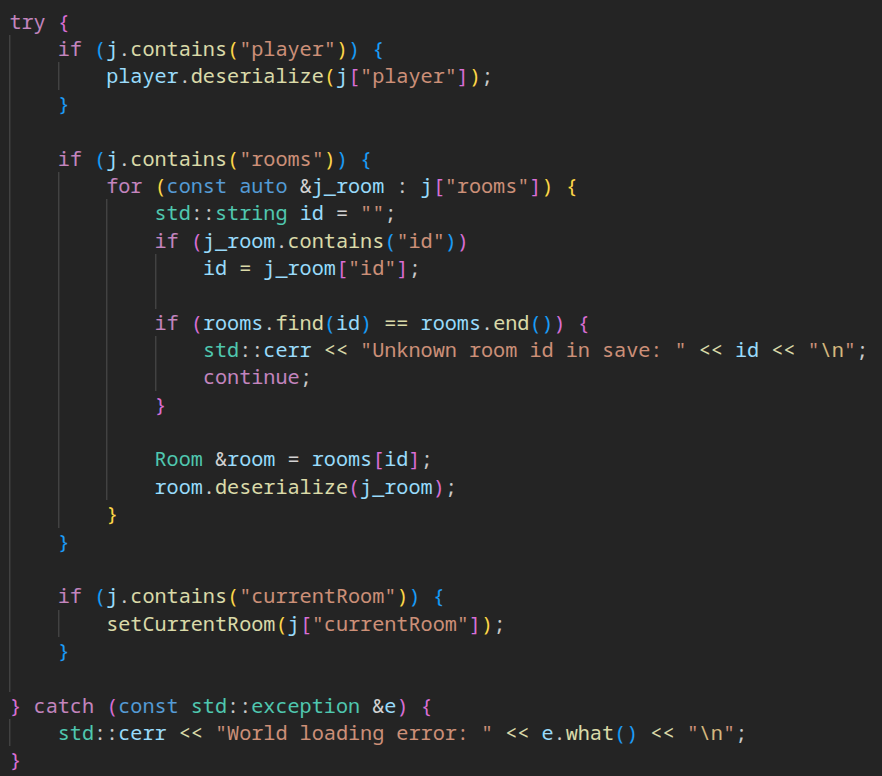
\includegraphics{_images/loadWorldData.png}
			\end{center}
		\end{column}
	\end{columns}
\end{frame}

\end{document}
